% !TEX root = MAIN.tex

\section{DAMAt}


\subsection{Software static architecture}

\begin{figure}[h]
  \centering
	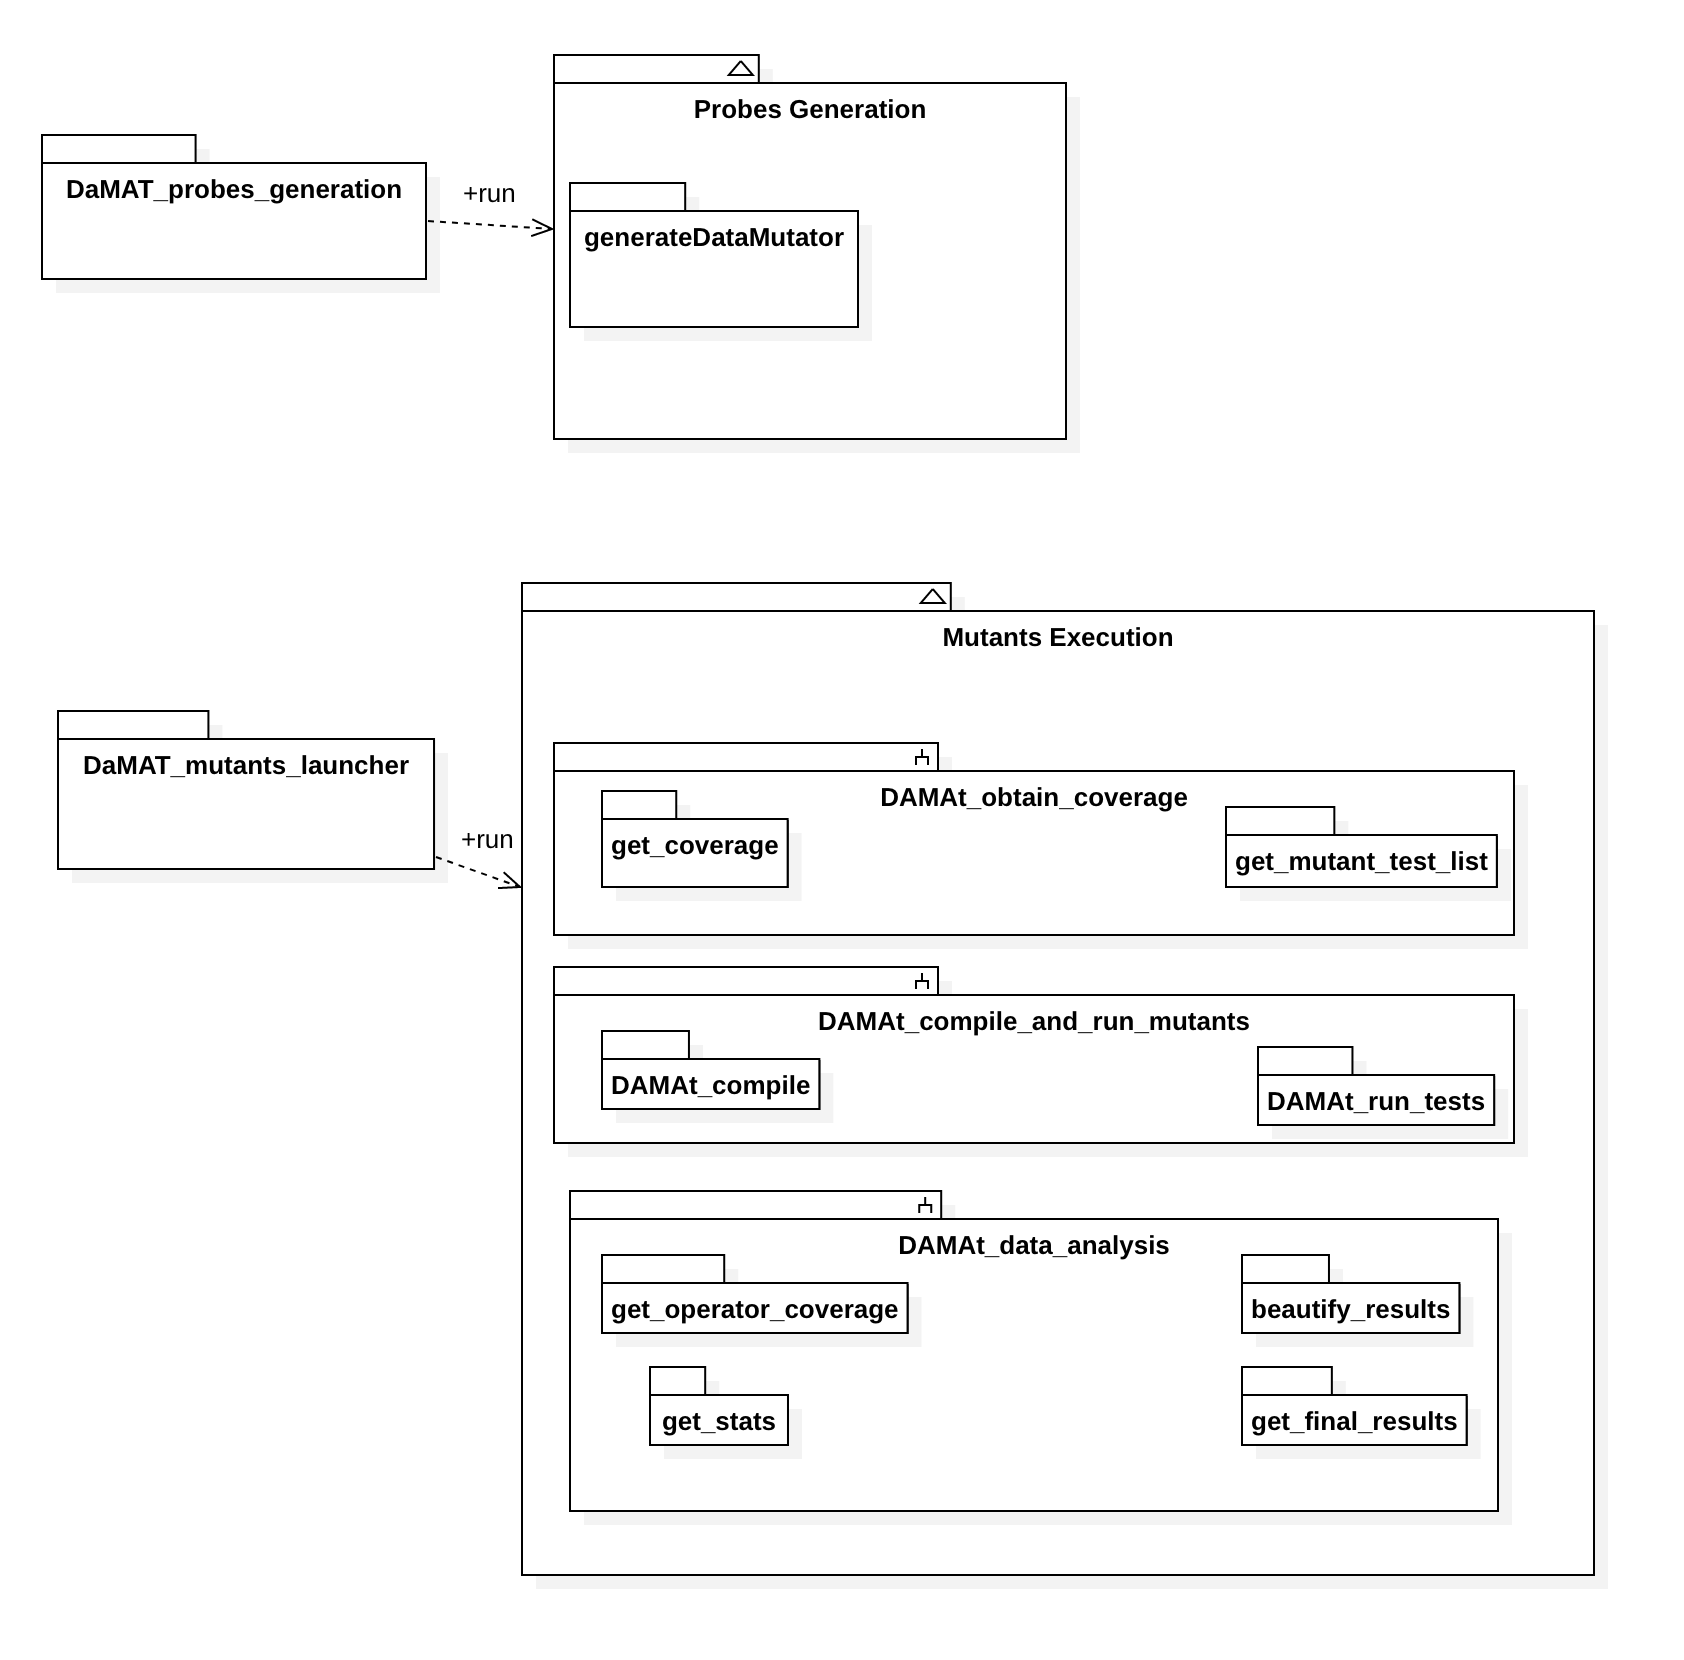
\includegraphics[width=0.8\textwidth]{images/damat_architecture_diagram.png}
      \caption{UML Architecture diagram of \dama.}
      \label{fig:damat_architecture_diagram}
\end{figure}

The architecture of the code-driven mutation analysis toolset (i.e., \dama)  is drafted in
Figure~\ref{fig:damat_architecture_diagram} relying on UML package diagram notation.

As depicted in Figure~\ref{fig:damat_architecture_diagram}, the architecture of the component is divided in two packages, which are named \textit{Probes Generation} and \textit{Mutants Execution} Also, it includes the two entry points:
\begin{itemize}
  \item \textit{damat\_probe\_generation}
  \item \textit{damat\_mutants\_launcher}
\end{itemize}

The package \textit{Probes Generation} implements the features concerning the generation of the data mutation API.

The package \textit{Mutants Execution} implements the features regarding the compilation and execution of mutants and the analysis of the results of the \dama procedure. Note that this layer implements also the strategies for the reduction of the test suite.

\subsubsection{Source Code Structure}


\dama is delivered as a compressed archive consisting of source files.
The following bullet points describe the archive's structure once uncompressed:

\begin{itemize}
	\item \textit{damat\_configure.sh}: this script defines the necessary variables for the execution of \dama. They shall be set by the engineer.
	\item \textit{damat\_probe\_generation.sh}: this script set the variables necessary to generate the data mutation API and execute the python script \textit{generateDataMutator.py} to generate them.
	\item \textit{damat\_mutants\_launcher.sh}: this script starts the \dama pipeline.
	\item \textit{generateDataMutator.py}: this is the script that generates the \dama mutation API.
	\item \textit{DDB\_TEMPLATE\_header.c} and \textit{DDB\_TEMPLATE\_footer.c}: these are templates used to generate the \dama API by \textit{generateDataMutator.py}
	\item \textit{damat\_compile.sh}: this is a stub of the script used to compile a mutant, which shall be completed by the engineer.
	\item \textit{damat\_run\_tests.sh}: this is a stub of the script used to run the tests, which shall be completed by the engineer.
	\item \textit{data\_analysis}: a folder containing five python scripts used for the generation of the final results:
	\begin{itemize}
	  \item \textit{beautify\_results.py}: this script renders the raw results from the execution of the tests in a more readable format.
	  \item \textit{get\_coverage.py}: this script analizes the results of the fault model coverage.
	  \item \textit{get\_operator\_coverage.py}: this script analizes the results of the operator coverage.
	  \item \textit{get\_stats.py}: this script produces statistics from the mutants' execution.
		\item \textit{get\_final\_results.py}: this script produces a summary of the execution of \dama.
	\end{itemize}
	\item \textit{pipeline\_scripts}: a folder containing the four scripts that make up the \dama pipeline:
	\begin{itemize}
		\item \textit{damat\_obtain\_coverage.sh}: this script obtains fault model coverage data in order to execute only the tests that cover each mutant.
		\item \textit{get\_mutant\_test\_list.py}: this script produces the list of test against which avery mutant shall be executed.
	  \item \textit{damat\_compile\_and\_run\_mutants.sh}: this scripts compile each mutant and run it against the SUT test suite.
		\item \textit{damat\_data\_analysis.sh}: this script executes all the data analysis steps at the end of the execution of the \dama pipeline
	\end{itemize}
	\item \textit{fault\_model.csv}: an example of a \dama fault model in csv format.
 	\item \textit{tests.csv }: an example of list of test cases and nominal times in csv format.
\end{itemize}
\clearpage

\subsection{Software components design}
\label{sec:damat_component:design}

\begin{figure}[tb]
  \centering
	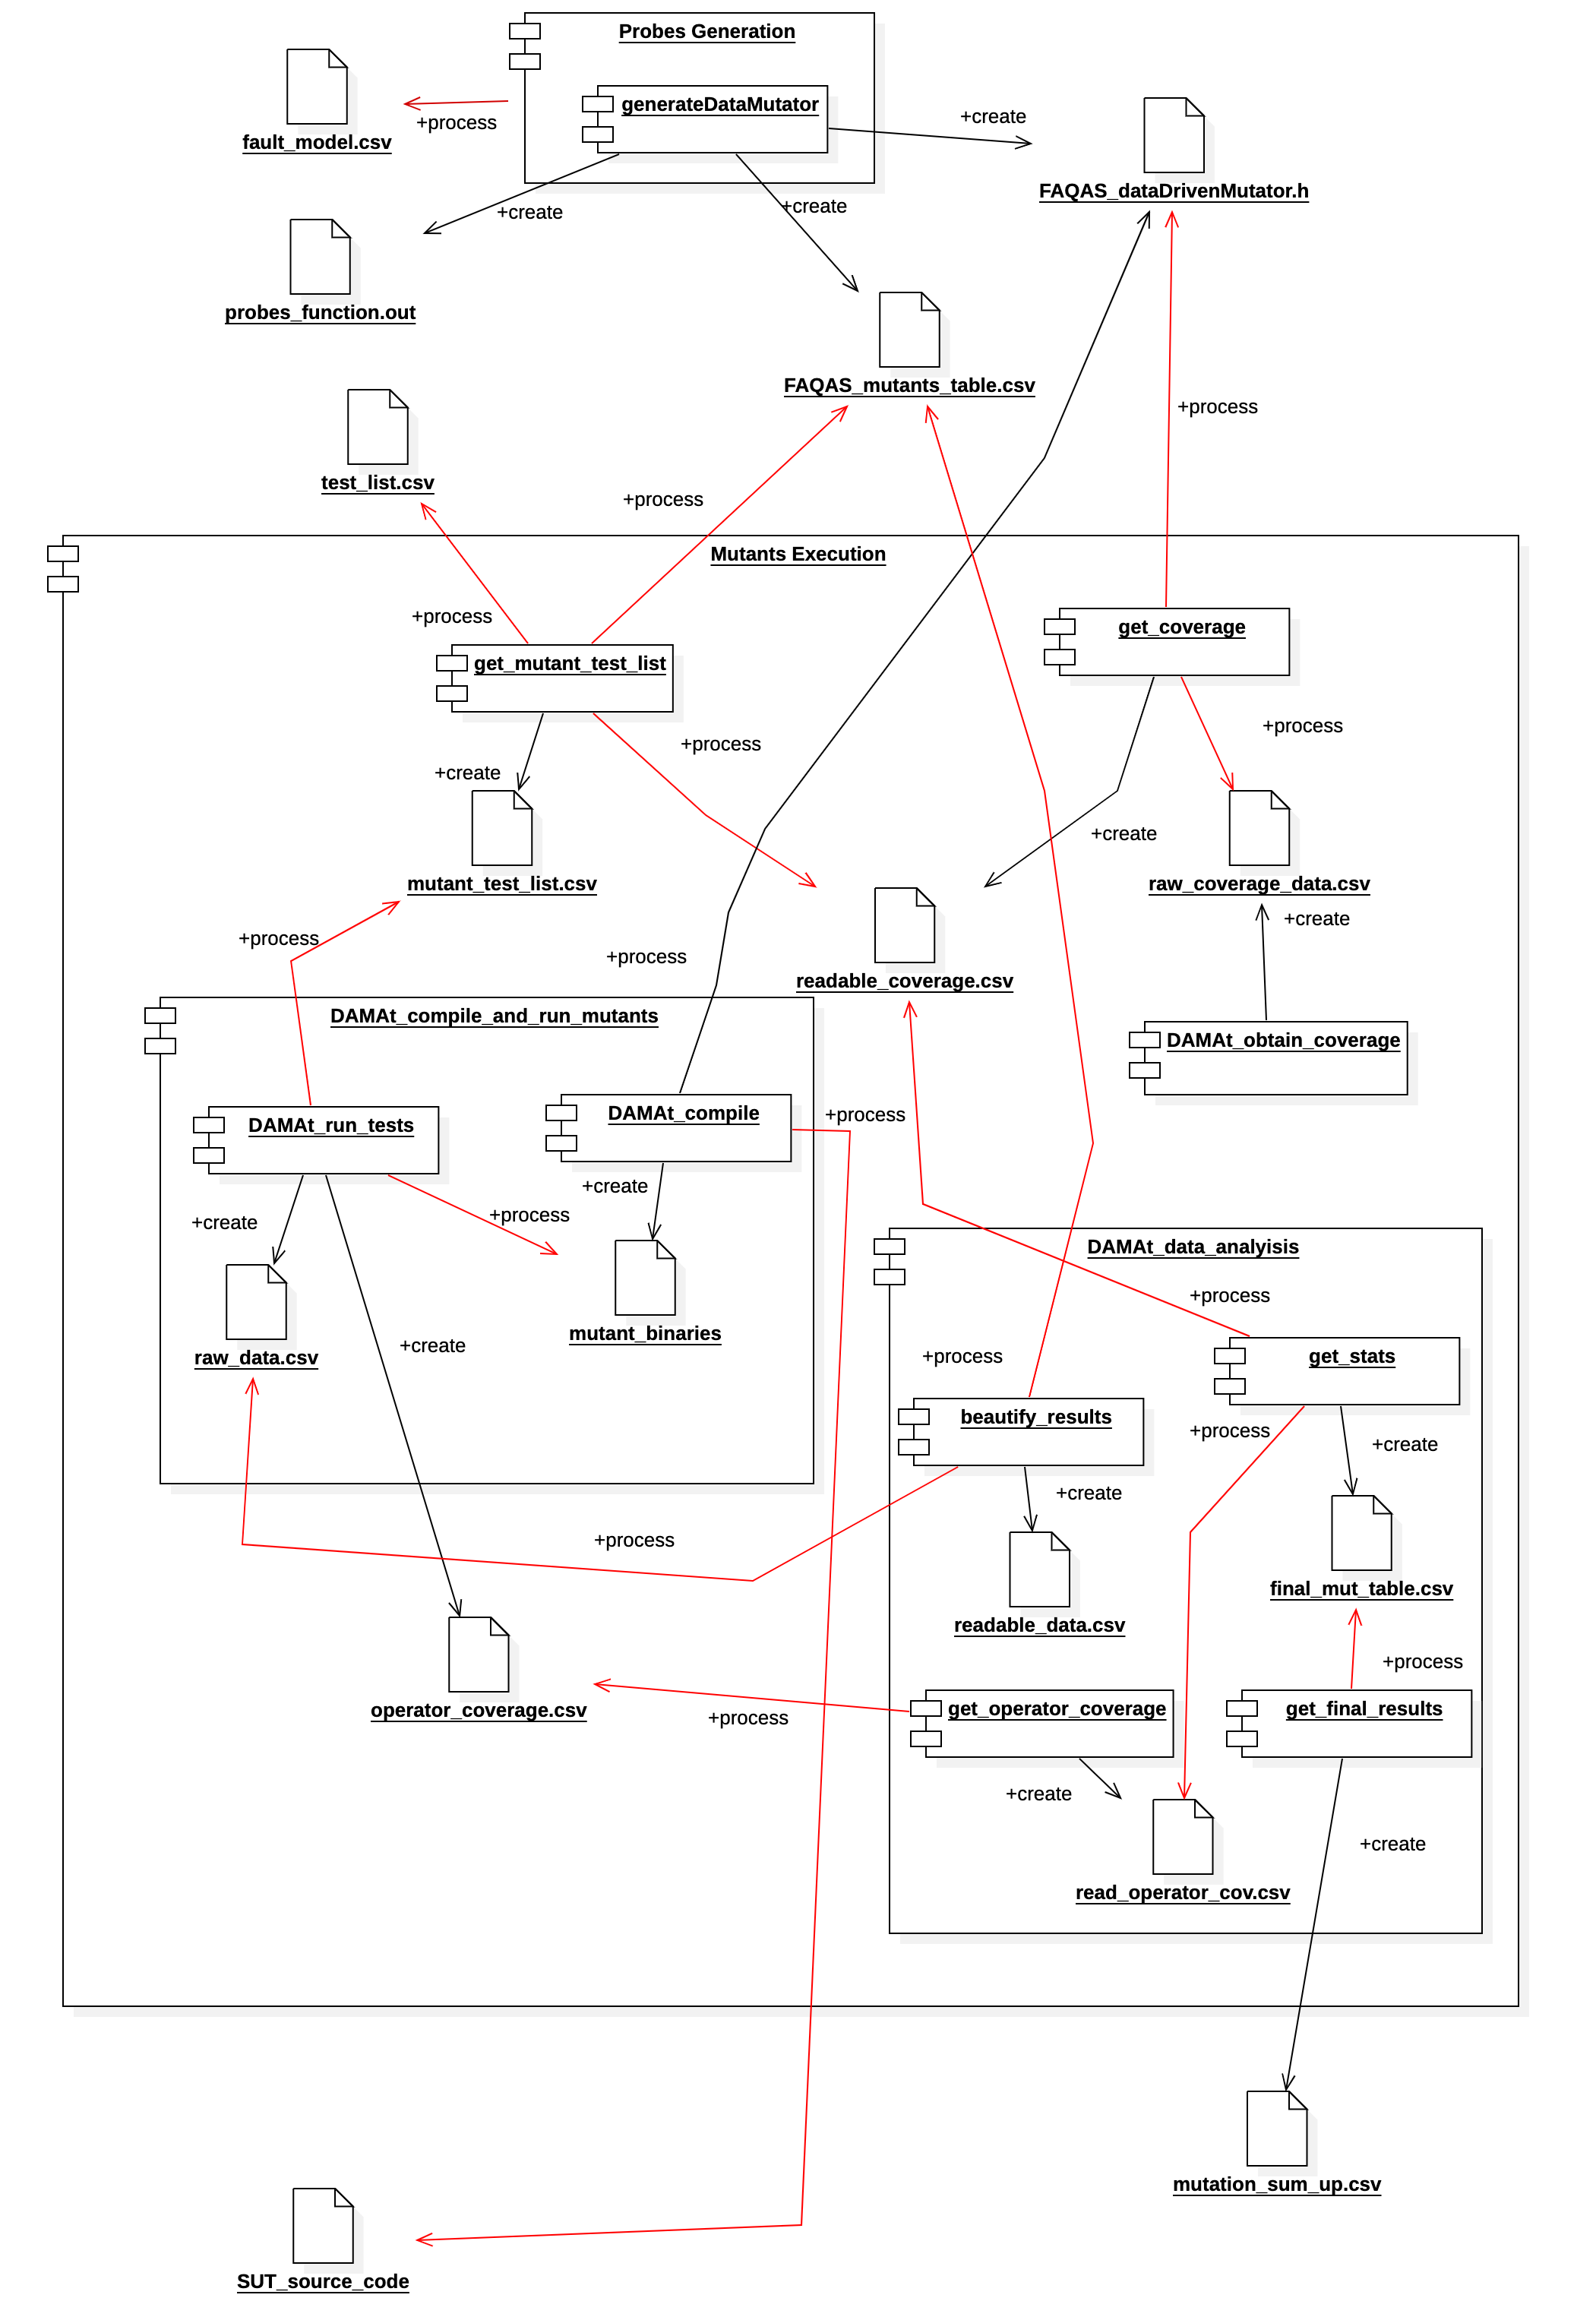
\includegraphics[width=0.9\textwidth]{images/damat_components.png}
      \caption{UML Component diagram of the data-driven mutation testing component to evaluate test suite effectiveness.}
      \label{fig:damat_component_diagram}
\end{figure}

The components of \dama are drafted in Figure~\ref{fig:damat_component_diagram}. Figure~\ref{fig:damat_component_diagram} relies on UML component diagram notation.

As shown in Figure~\ref{fig:damat_component_diagram}, the software is composed by the following components:

\begin{itemize}
  \item \textit{fault\_model.csv}: this csv file shall be provided by the engineer and contains one row for every mutation operator. Every mutation operator shall generate one or more mutants.
  For details see D2. An example of line is:

  \texttt{fault\_model\_01,0,1,BIN,BF,3,3,NA,NA,-1,1}

  \item \textit{test\_list.csv}: this csv file shall be provided by the engineer and contains one row per test case, containing an identifier for the test and the average time of execution expressed in ms. An example of a line is:

  \texttt{test\_01,34598}

  \item \textit{Probe  Generation}: this component processes the fault model and and generates \textit{FAQAS\_dataDrivenMutator.h}, \textit{FAQAS\_mutants\_table.csv}  and \textit{probes\_function.out}
  \item \textit{FAQAS\_dataDrivenMutator.h}: this is the API that contains the logic for the data drive mutation.
  \item \textit{FAQAS\_mutants\_table.csv}: this is a csv file containing the definition and \texttt{MutationOpt} (a mumerical ID) for every generated mutant. Every row represents a generated mutant. This is an example of a row:

  \texttt{0,fault\_model\_01,0,1,BIN,BF,3,3,NA,NA,-1,1}

  \item \textit{probes\_function.out}: this file contains prototypes for the mutation probes, which are calls to functions defined in the mutation API.
  \item \textit{Mutants Execution}: this component contains subcomponents that handle the test suite reduction, compilation, execution and data gathering relative to the execution of \dama.
  \begin{itemize}
    \item \textit{DAMAt\_obtain\_coverage}: this component executes a special mutant against the test suite that collects the \textit{raw\_coverage\_data.csv} file.

    \item \textit{raw\_coverage\_data.csv}: this file is a collection of the coverage data for each test. A row is produced every time a mutation function is called. It contains a numerical ID relative to the fault model.
    This is an example of row:

    \texttt{fm.ID: 0}

    \item \textit{get\_coverage}: this component process the \textit{raw\_coverage\_data.csv} file to produce \textit{readable\_coverage\_data.csv}.

    \item \textit{readable\_coverage\_data.csv}: this file is a collection of the coverage data for each couple test-fault model in a more accessible and compact format.
    This is an example of row:

    \texttt{test\_01,fault\_model\_01,<coverage status>,<nr of calls>}

    \item \textit{get\_mutant\_test\_list}: this component processes \textit{test\_list.csv} and \textit{readable\_coverage\_data.csv} to produce \textit{mutant\_test\_list.csv}.

    \item \textit{mutant\_test\_list.csv} is a csv file containing a reduced version of \textit{test\_list.csv} specific for every mutant with only the tests covering that specific mutant. The structure is the same as \textit{test\_list.csv}.

    \item \textit{DAMAt\_compile\_and\_run\_mutants}: this component contains subcomponents that compile the generated mutants and run them against the test suite of the SUT.
    \begin{itemize}
      \item \textit{DaMAT\_compile}: this component processes \textit{FAQAS\_dataDrivenMutator.h} and the \textit{SUT source code} to produce the \textit{mutant binary files}.
      \item \textit{DAMAt\_run\_tests}: this component processes the \textit{mutant binary files} and the \textit{mutant\_test\_list.csv}, producing \textit{raw\_data.csv} and \textit{operator\_coverage.csv}.
      \item \textit{raw\_data.csv} is a file in the csv format. Each row contains the result of the execution of a mutant against a test case.
      This is an example:

      \begin{lstlisting}
      <mutationOpt>;COMPILED;test_01;PASSED;LIVE;<elapsed time>
      <mutationOpt>;COMPILED;test_02;FAILED;KILLED;<elapsed time>
      \end{lstlisting}

      \item \textit{operator\_coverage.csv}: this is a file in the csv format. Every row describes a call to the mutation API. The first column contains a sequential index that identifies the call and the second row contains \texttt{1} if the mutation operator was successfully applied or \texttt{0} if not.
      This is an example or a row:

      \texttt{234,0}

    \end{itemize}
    \item \textit{DAMAt\_data\_analysis}: this component contains subcomponents that analise the data produced from an execution of \dama and produce the final results.
    \begin{itemize}
      \item \textit{beautify\_results}: this component processes \textit{raw\_data.csv} and \textit{FAQAS\_mutants\_table.csv} to produce \textit{readable\_data.csv}
      \item \textit{readable\_data.csv} is a more complete csv. Every row represents a mutant-test case couple and contains the definition of the mutant.
      An example is provided below:

      \begin{lstlisting}
      <mutationOpt>,COMPILED,test_01,PASSED,LIVE,36378,fault_model_01,0,1,BIN,BF,3,3,NA,NA,-1,1
      <mutationOpt>,COMPILED,test_02,PASSED,LIVE,43364,fault_model_02,28,2,DOUBLE,VOR,-20,50,NA,1,NA,NA
      \end{lstlisting}

      \item \textit{get\_operator\_coverage} this component processes  \textit{operator\_coverage.csv} to produce \textit{readable\_operator\_coverage.csv}
      \item \textit{readable\_operator\_coverage.csv}: this cvs file is a rendition of /\textit{operator\_coverage.csv} in a more compact and undertandable format.
      every row represent a mutant-test case couple. the srtucture is provoded below

      \texttt{<MutationOpt>,<testID>,<nr of calls>,<number of successful application>}

      \item \textit{get\_stats} this component processes \textit{readable\_coverage.csv}, \textit{readable\_operator\_coverage.csv} and \textit{readable\_data.csv} to produce \textit{final\_mutants\_table.csv}
      \item \textit{final\_mutants\_table.csv} is a file in the csv format that contains a row for every mutant. Every row contains informations about the mutant definition and status.
      An example is provided below:

      \begin{lstlisting}
      <MutationOpt>,fault_model_01,0,1,BIN,BF,3,3,NA,NA,-1,1,LIVE,APPLIED
      <MutationOpt>,fault_model_02,0,1,BIN,BF,4,4,NA,NA,-1,1,NOT_COVERED,NOT_APPLIED
      \end{lstlisting}

      \item \textit{get\_final\_results}: this component processes \textit{final\_mutants\_table.csv} to produce \textit{mutation\_sum\_up.csv}
      \item \textit{mutation\_sum\_up.csv} is a csv file that contains a summary of the execution of \dama.
      An example is provided below:

      \begin{lstlisting}
      all_fault_models,covered_fault_models,fault_model_coverage
      11,2,0.182
      covered_mutants,applied_mutants,operator_coverage
      2,2,1.0
      applied_mutants,killed_mutants,mutation_score
      2,0,0.0
      \end{lstlisting}

    \end{itemize}
  \end{itemize}

\end{itemize}
\clearpage


\begin{figure}[h]
  \centering
	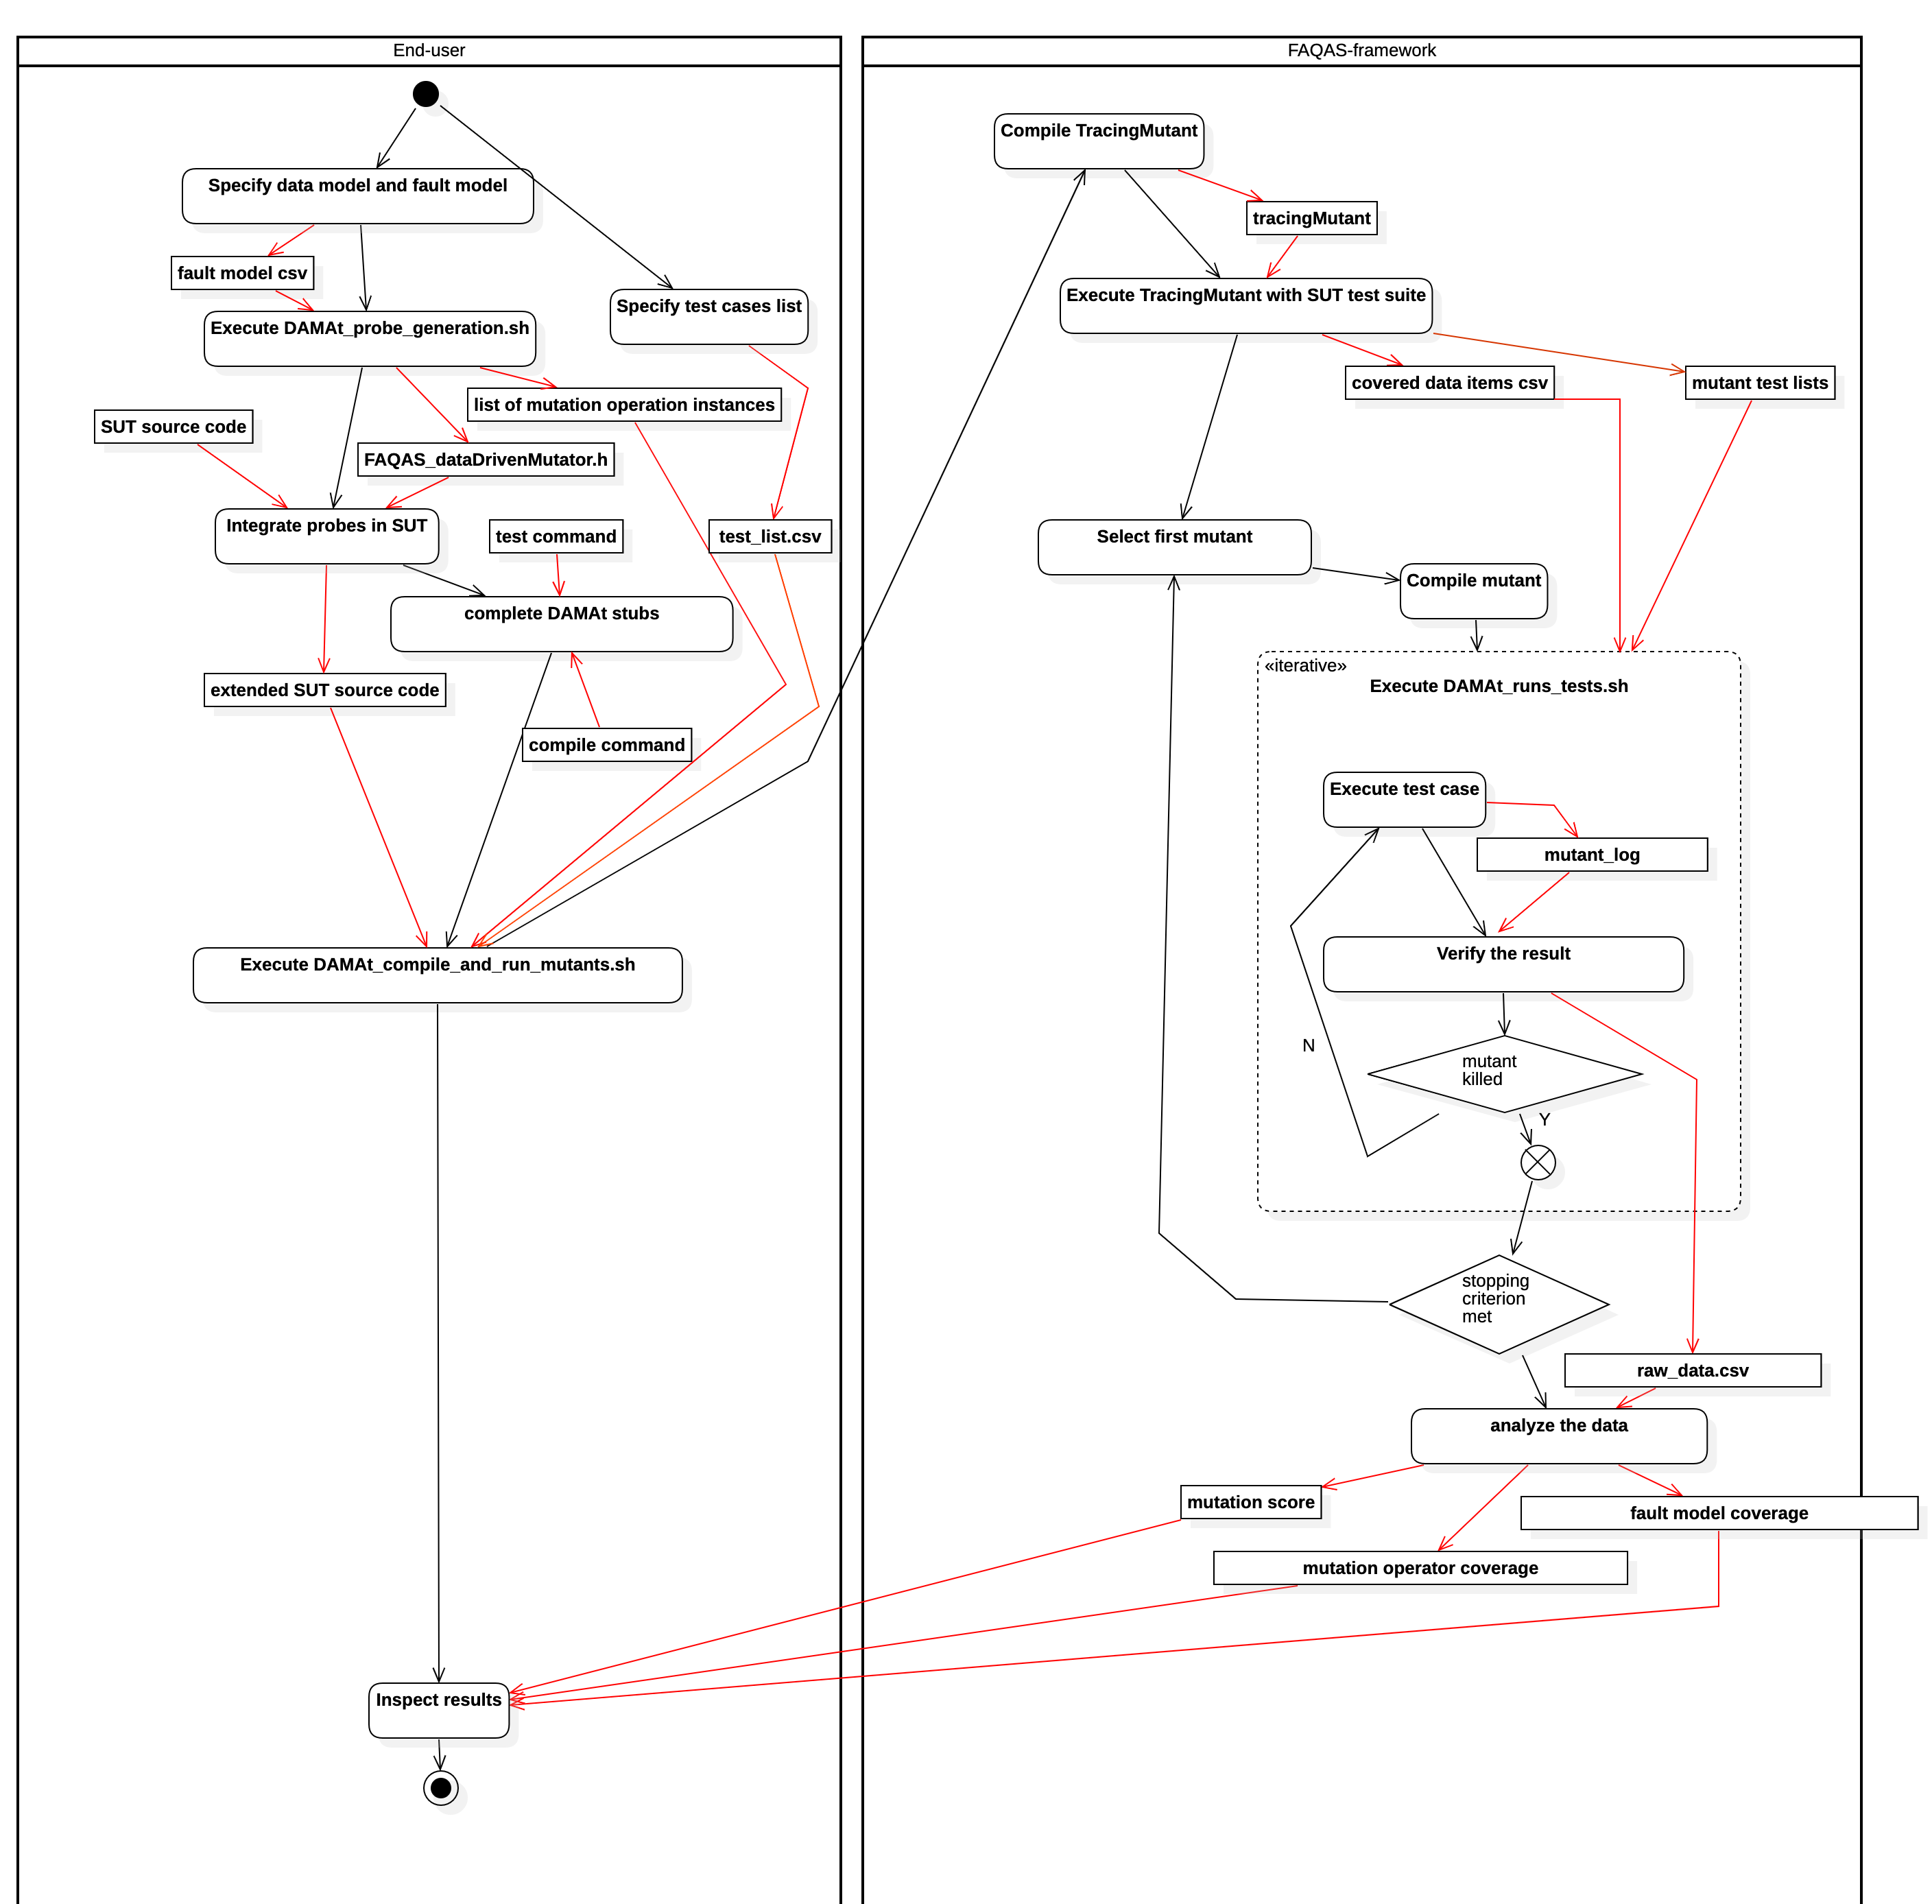
\includegraphics[width=\textwidth]{images/png/data_driven_process.png}
      \caption{Overview of the data-driven mutation testing process to evaluate test suite effectiveness.}
      \label{fig:process:dataDriven:evaluation}
\end{figure}
%
\dama implements the process for the evaluation of test suite effectiveness that is drafted in Figure~\ref{fig:process:dataDriven:evaluation}. Figure~\ref{fig:process:dataDriven:evaluation} relies on UML activity diagram notation. In Figure~\ref{fig:process:dataDriven:evaluation} the execution of specific software artifacts by the end-user is made explicit. Also, we use black arrows to draw control flow, red arrows for data flow.

The activity \emph{Specify data model and fault model} in Figure~\ref{fig:process:dataDriven:evaluation} indicates that the engineer should prepare a csv file specifying the fault model and the data model for the SUT according to D2.

The activity \emph{Specify test cases list} in Figure~\ref{fig:process:dataDriven:evaluation} indicates that the engineer should prepare a csv file specifying the name and nominal time of all test cases.

The activity \emph{Execute \dama\_probe\_generation.sh} in Figure~\ref{fig:process:dataDriven:evaluation} concerns the execution of the program \emph{\dama\_probe\_generation.sh}.

The program \emph{\dama\_probe\_generation.sh} takes as input the \emph{fault model csv} and generates the file \emph{FAQAS\_dataDrivenMutator.h} and a csv file containing the \emph{list of mutation operation instances} derived from the fault model.

File \emph{FAQAS\_dataDrivenMutator.h} contains the FAQAS mutation testing API (i.e., the predefined functions to perform data mutation for buffers) and the fault model represented as a data structure. Details are provided in D2.

The activity \emph{Integrate probes in SUT} in Figure~\ref{fig:process:dataDriven:evaluation} indicates that the engineer should manually modify the source code of the SUT to integrate mutation probes into it. Examples are provided in \emph{Listing 2.3}, \emph{Listing 3.1}, and \emph{Appendix A - Section 1.1} of D2.

The activity \emph{complete \dama stubs} in Figure~\ref{fig:process:dataDriven:evaluation} indicates that the engineer is expected to manually integrate the compilation and execution stubs provided by \dama with the commands used for compiling the SUT and executing test cases after the execution of every single test case.

The activity \emph{Execute \dama\_compile\_and\_run\_mutants.sh} in Figure~\ref{fig:process:dataDriven:evaluation} concerns the execution of the program \emph{\dama\_compile\_and\_run\_mutants.sh}

The program \emph{\dama\_compile\_and\_run\_mutants.sh.} automatically executes a number of activities required to compute the mutation score: \emph{Compile TracingMutant}, \emph{Execute TracingMutant with SUT test suite}, \emph{Select first mutant}, \emph{Compile mutant}, \emph{Execute test case},  \emph{analyze the data}.

The activity \emph{Compile TracingMutant} indicates that the system compiles a version of the SUT that traces the data items (targeted by mutation) that are covered by each test case (see D2, Figure 2.9, line 5).

The activity \emph{Execute TracingMutant with SUT test suite} indicates that the system executes the SUT test suite. Since the test suite is executed with the TracingMutant it leads to the generation of a csv file that indicates, for every test case, the data items being exercised by the test case.

The activity \emph{Select first mutant} indicates that  \emph{FAQAS-CompileAndExecuteMutants} selects the first item in the \emph{list of mutation operation instances} and removes it from the list.

The activity \emph{Compile mutant} indicates that the system compiles a version of the SUT with the selected mutation operation instance enabled.

The activity \emph{Execute test case} indicates that the test suite of the SUT executes a test case. Only the test cases exercising the data item targeted by the mutation operator are executed. Since the test case is executed against the mutated SUT, if the mutation operation is performed, then the file \emph{mutant\_log} will be created (this is a feature of the FAQAS data-driven mutation API).

File \emph{mutant\_log} contains the ID of the mutation operation instance applied.

The activity \emph{Verify the result} receives as input the ID of the test case and the status of a test case (i.e., PASS or FAIL). It checks if a data mutation operator has been applied based on the content of \emph{mutant\_log}. It updates the content of \emph{raw\_data.csv}

If program \emph{Verify the result} determines that a mutation operation instance has been killed, then the test suite execution is terminated.

File \emph{raw\_data.csv} indicates, for every executed test case, the ID of the mutation operation instance applied and the mutation result (KILLED or LIVE). A test case may appear multiple times in this file, each time with a different mutation operation instance ID associated.

The execution of the test suite is repeated till a termination criterion is met. The termination criterion is the execution of all covered mutants.

The activity \emph{analyze the data} concerns the computation of the data-driven mutation metrics based on the mutation results reported in \emph{raw\_data.csv}:
\begin{enumerate}
	\item Fault model coverage is the percentage of fault models covered by the test suite.
	\item Mutation operation coverage is the percentage of data items that have been mutated at least once, considering only those that belong to the data buffers covered by the test suite.
	\item The mutation score (MS) is the percentage of mutants killed by the test suite (i.e., leading to at least one test case failure) among the mutants that target a fault model and for which at least one mutation operation was successfully performed.
\end{enumerate}
More information on these metrics is given in D2.
The end-user inspects these metrics to respectively take notice of these kinds of problems in the test suite:
\begin{enumerate}
	\item the message type targeted by a mutant is never exercised.
	\item the message type is covered by the test suite but it is not possible to perform some of the mutation operations.
	\item the mutation is performed but the test suite does not fail.
\end{enumerate}
\subsection{Internal interface design}



All the programs that automate the different steps of \MASS communicate only through the files that had been described in Section~\ref{sec:damat_component:design}.

\subsection{External interface design}

The external interfaces of the \MASS are the programs that automate the different steps of \MASS, which have been described above. They are

\begin{itemize}
  \item \texttt{DAMAt\_probe\_generation.sh}: which generates the mutation API.
	\item \texttt{DAMAt\_compile\_and\_run\_mutants.sh}: which executes the \dama pipeline.
\end{itemize}

\subsection{Test harness}

\dama provide unit test cases for the \texttt{FAQAS\_dataDrivenMutation} component that generate mutants from the SUT source code. More information can be found in the \textit{ESA-FAQAS-SUITP} document.
